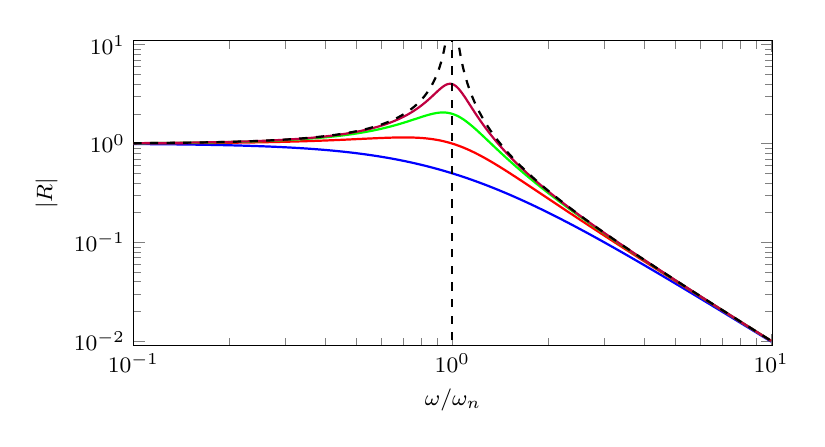
\begin{tikzpicture}[scale=1]
	\footnotesize
	\begin{axis}[
		width=0.8\textwidth,
		height=0.45\textwidth,
		xlabel={$\omega/\omega_n$},
		ylabel = {$|R|$},
		xmax=10.1,
		xmin=0.1,
		ymax=11,
		ymin=0.009 ,
		samples=1000,
		xmode=log,
		ymode=log]
		
		
		\def\k{1};
		\def\zetaA{1};
		\def\zetaB{0.5};
		\def\zetaC{0.25};
		\def\zetaD{0.125};		
		\def\zetaE{0.01};		
		
		\addplot[blue, thick, domain=0.1:10] (x, {1/sqrt(\k^2*(1-(x)^2)^2 + (\zetaA*2*\k*(x))^2)});
		\addplot[red, thick, domain=0.1:10] (x, {1/sqrt(\k^2*(1-(x)^2)^2 + (\zetaB*2*\k*(x))^2)});		
		\addplot[green, thick, domain=0.1:10] (x, {1/sqrt(\k^2*(1-(x)^2)^2 + (\zetaC*2*\k*(x))^2)});		
		\addplot[purple, thick, domain=0.1:10] (x, {1/sqrt(\k^2*(1-(x)^2)^2 + (\zetaD*2*\k*(x))^2)});		
		\addplot[black, dashed, thick, domain=0.1:10] (x, {1/sqrt(\k^2*(1-(x)^2)^2 + (\zetaE*2*\k*(x))^2)});		
		
		% Marks for damped resonance
%		\addplot[green, mark=*, domain=0.1:10] ({sqrt(1-2*\zetaC^2)}, {1/sqrt(\k^2*(1-(sqrt(1-2*\zetaC^2))^2)^2 + (\zetaC*2*\k*(sqrt(1-2*\zetaC^2)))^2)});
%		\addplot[purple, mark=*, domain=0.1:10] ({sqrt(1-2*\zetaD^2)}, {1/sqrt(\k^2*(1-(sqrt(1-2*\zetaD^2))^2)^2 + (\zetaD*2*\k*(sqrt(1-2*\zetaD^2)))^2)});
		
		\draw [thick, dashed] (axis cs: 1, 0.001) -- (axis cs: 1,11);

		
	\end{axis}
	
\end{tikzpicture}